%   FILE: foo.tex -- 
% AUTHOR: W. Michael Petullo <mike@flyn.org>
%   DATE: 25 October 2013
%
% Copyright (C) 2013 W. Michael Petullo <mike@flyn.org>
% All rights reserved.

\documentclass{article}

\usepackage{pdflscape}
\usepackage{booktabs}
\usepackage{listings}
\usepackage{paralist}
\usepackage{pgfgantt}
\usepackage{fullpage}
\usepackage[group-separator={,},group-minimum-digits=3,round-mode=places,round-precision=2]{siunitx}
\usepackage{todonotes}
\usepackage{url}
\usepackage{verbatim}
\usepackage{xfrac}

\newcommand{\command}[1]{{\sffamily#1}}
\newcommand{\class}[1]{{\sffamily#1}}
\newcommand{\procedure}[1]{{\sffamily#1}}
\newcommand{\configOption}[1]{{\sffamily#1}}
% NOTE: also used as values:
\newcommand{\variable}[1]{{\sffamily#1}}
\newcommand{\unix}{\textsc{Unix}\xspace}
\newcommand{\figref}[1]{Figure~\ref{#1}}
\newcommand{\apref}[1]{Appendix~\ref{#1}}

\usetikzlibrary{decorations.pathmorphing}
\tikzstyle{highlighter} = [
	orange,
	line width = \baselineskip,
	opacity=0.25,
	decorate,
	decoration = random steps
]

\newcommand\bh{\tikz[remember picture]\coordinate(begin highlight){};}
\newcommand\eh{\tikz[remember picture]\coordinate(end highlight){};\tikz[remember picture,overlay]\draw[highlighter]([shift={(0,0.5ex)}]begin highlight)--([shift={(0,0.5ex)}]end highlight);}

% Implementation of the core highlighting logic; do not change!
%\newcounter{highlight}[page]
%\newcommand{\tikzhighlightanchor}[1]{\ensuremath{\vcenter{\hbox{\tikz[remember picture, overlay]{\coordinate (#1 highlight \arabic{highlight});}}}}}
%\newcommand{\bh}[0]{\stepcounter{highlight}\tikzhighlightanchor{begin}}
%\newcommand{\eh}[0]{\tikzhighlightanchor{end}}
%\AtBeginShipout{\AtBeginShipoutUpperLeft{\ifthenelse{\value{highlight} > 0}{\tikz[remember picture, overlay]{\foreach \stroke in {1,...,\arabic{highlight}} \draw[highlighter] (begin highlight \stroke) -- (end highlight \stroke);}}{}}}

\lstMakeShortInline[basicstyle=\small\sffamily,columns=fullflexible]|

\lstdefinestyle{commands}{%
        basicstyle=\sffamily\footnotesize,
	backgroundcolor=\color{highlightYellow},
	columns=fullflexible,
        frame=single,
        tabsize=8,
        % Note: each line in listing should start with 3*tab.
        escapeinside={(*}{*)},
        % Next line affects alignment in big figure/subfigures.
        breaklines=true,
        breakatwhitespace=true,
	aboveskip=3pt,
	belowskip=3pt,
}

\lstdefinestyle{java}{%
	basicstyle=\sffamily\footnotesize,
	backgroundcolor=\color{highlightYellow},
	columns=fullflexible,
	language=c,
	frame=single,
	tabsize=8,
	numbers=left,
	numberblanklines=false,
	% Note: each line in listing should start with 4*space.
	numbersep=-1.3em,
	escapeinside={(*}{*)},
	% Next line affects alignment in big figure/subfigures.
	breaklines=true,
	breakatwhitespace=true,
	framesep=0em,
	framexleftmargin=3pt,
	framexrightmargin=3pt,
	framextopmargin=3pt,
	framexbottommargin=1pt,
	aboveskip=3pt,
	belowskip=0pt,
	numberstyle=\scriptsize
}

\lstdefinestyle{c}{%
	basicstyle=\sffamily\footnotesize,
	backgroundcolor=\color{highlightYellow},
	columns=fullflexible,
	language=c,
	frame=single,
	tabsize=8,
	numbers=left,
	numberblanklines=false,
	% Note: each line in listing should start with 4*space.
	numbersep=-1.3em,
	escapeinside={(*}{*)},
	% Next line affects alignment in big figure/subfigures.
	breaklines=true,
	breakatwhitespace=true,
	framesep=0em,
	framexleftmargin=3pt,
	framexrightmargin=3pt,
	framextopmargin=3pt,
	framexbottommargin=1pt,
	aboveskip=3pt,
	belowskip=0pt,
	numberstyle=\scriptsize
}

\lstdefinestyle{pseudo}{%
	basicstyle=\sffamily\footnotesize,
	backgroundcolor=\color{highlightYellow},
	columns=fullflexible,
	frame=single,
	tabsize=8,
	numbers=left,
	numberblanklines=false,
	% Note: each line in listing should start with 4*space.
	numbersep=-1.3em,
	escapeinside={(*}{*)},
	% Next line affects alignment in big figure/subfigures.
	breaklines=true,
	breakatwhitespace=true,
	framesep=0em,
	framexleftmargin=3pt,
	framexrightmargin=3pt,
	framextopmargin=3pt,
	framexbottommargin=1pt,
	numberstyle=\scriptsize,
	aboveskip=3pt,
	belowskip=0pt,
	literate=
               {...}{{\ldots}}1
               {=}{{$\gets$}}1
               {<=}{{$\leq$}}1
               {>=}{{$\geq$}}1
               {!=}{{$\neq$}}1
               {==}{{=}}1
}

% For use with paralist/inparaenum.
\setdefaultenum{(1)}{(a)}{i)}{}

\pdfpagewidth 8.5in
\pdfpageheight 11in

\title{Project Phase 5: \\ Analysis of two Nachos Schedulers}
\author{W. Michael Petullo}

\begin{document}

\maketitle

\section{Nachos process states}
Figure~\ref{fig:states} shows a graph where the nodes are the process
states implemented by Nachos, and the edges are allowed state transitions.
Also depicted are the methods from Nachos' \command{KThread} class
to which I added instrumentation code. 

\begin{figure}[h]
\centering
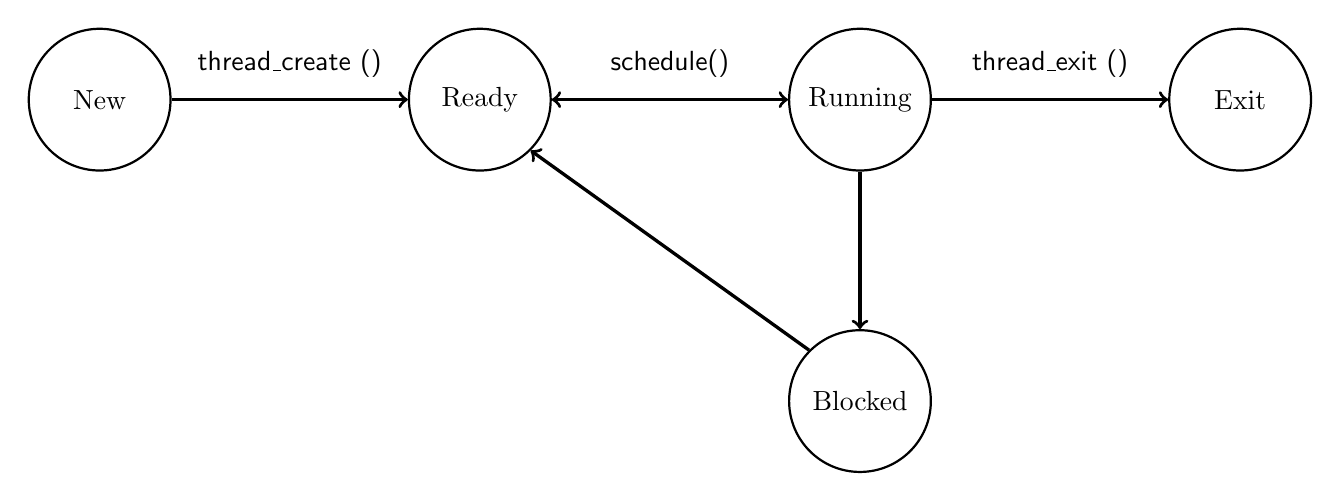
\begin{tikzpicture}
\draw (0,0) node[draw,circle,fill=white,thick,minimum size=1.8cm] (ready) {Ready};
\node[draw,circle,fill=white,thick,minimum size=1.8cm] (new) [left=3cm of ready] {New};
\node[draw,circle,fill=white,thick,minimum size=1.8cm] (running) [right=3cm of ready] {Running};
\node[draw,circle,fill=white,thick,minimum size=1.8cm] (exit) [right=3cm of running] {Exit};
\node[draw,circle,fill=white,thick,minimum size=1.8cm] (blocked) [below=2cm of running] {Blocked};

\draw[very thick,->] (node cs:name=new,angle=0) -- node[label=above:\textsf{thread\_create ()}] {} (node cs:name=ready,angle=180);
\draw[very thick,->] (node cs:name=running,angle=0) -- node[label=above:\textsf{thread\_exit ()}] {} (node cs:name=exit,angle=180);
\draw[very thick,<->] (node cs:name=ready,angle=0) -- node[label=above:\textsf{schedule()}] {} (node cs:name=running,angle=180);
\draw[very thick,->] (node cs:name=running,angle=270) -- node {} (node cs:name=blocked,angle=90);
\draw[very thick,->] (node cs:name=blocked,angle=135) -- node {} (node cs:name=ready,angle=315);

\end{tikzpicture}
\caption{The basic Nachos state graph; Nodes represent states, and edges represent allowed transitions}
\label{fig:states}
\end{figure}

\section{Instrumentation}
I added instrumentation code to the methods indicated in Figure~\ref{fig:states}.
Each routine outputs the data described below to the system console.

The instrumentation code prints lines of the following form:
\begin{center}
\command{MEASUREMENT $p$ (\#$i$) a: $a$ s: $s$ e: $e$},
\end{center}
where
\begin{description}
\item[\textnormal{MEASUREMENT}] is a magic string to differentiate between measurements and other output,
\item[$p$] is a program name (e.g., \command{count-looper}),
\item[$i$] is the corresponding process ID,
\item[$a$] indicates the arrival time of $p$ (from \procedure{thread\_create}),
\item[$s$] indicates a time at which process $p$ began executing on the processor (from \procedure{schedule}), and
\item[$e$] indicates the exit time of $p$ (from \procedure{thread\_exit}).
\end{description}
Time is recorded as ticks,
and each of $a$, $s$, and $e$ might be -1, depending on which value was measured for a particular record.
Thus
\begin{center}
\begin{tabular}{l}
\command{count-looper (\#3) a: 1 s: -1 e: -1} \\
\command{count-looper (\#3) a: -1 s: 2 e: -1} \\
\command{shell (\#2) a: -1 s: 3 e: -1} \\
\command{count-looper (\#2) a: -1 s: -1 e: 4}
\end{tabular}
\end{center}
shows that the loaded submitted \command{count-looper} for execution at tick 1,
the processor began executing \command{count-looper} at tick 2,
\command{sh} resumed executing at tick 3 (replacing \command{count-looper} in the running state),
and \command{count-looper} exited at tick 4.

\section{Scheduler description}

Pintos has a notion of time that is based on \emph{ticks}. Each timer interrup
advances the tick counter by one tick.

The round-robin scheduler provides support for interactive processes,
where a user can run and manipulate several programs concurrently.
Pintos maintains a linked-list queue of ready processes,
and these processes run using the following algorithm:
\begin{enumerate}
\item Pintos removes the process at the head of the list and sets it to run on the processor.
\item The process runs until either
\begin{inparaenum}
\item the timer goes off and Pintos moves the process to the tail of the ready list or
\item the process makes a blocking system call.
\end{inparaenum}
\item In either case, Pintos returns to step (1).
\end{enumerate}
Because I/O-bound processes will not make use of their entire time quantum
(i.e., they will give up a portion of their time quantum upon making a blocking I/O call),
they are at a disadvantage when compared to CPU-bound processes.

Pintos' round-robin scheduler is appropriate for an interactive system,
and has the following properties with respect to our textbook's scheduling criteria:
\begin{description}
\item[Response time] Processes should remain responsive when using
the round-robin scheduler, because the timer will go off every 500
instructions. One downside of the Nachos architecture (as described when
I introduced ticks above) is that there is a degree of unpredictability
resulting from time progressing by a fixed degree while the Nachos kernel
is executing, independent of how much wall-clock time a kernel function
takes.

\item[Deadlines] The round-robin scheduler does not support deadlines.
There is no facility allowing one to change the scheduling discipline
in order to get a process to complete before a certain time.

\item[Predictability] Once a process begins running, it is difficult to predict how long it will take for it to complete.
A system with $n$ processes will run each at approximately \sfrac{1}{n} the rate that they would run on a dedicated computer.
Furthermore, the overhead of performing context switches will degrade performance,
due especially because of TLB flushing, cache invalidations, and direct context-switch overhead.

\item[Throughput] The round-robin scheduler should provide good
throughput, although performance of each process will be affected as
described for predictability.

\item[Processor utilization] The round-robin scheduler should make good use of the processor.

\item[Fairness] The round-robin scheduler does not introduce the possibility of starvation.

\item[Enforcing priorities] The round-robin scheduler does not provide support for process priorities.

\end{description}

\section{Experiment design and analysis}

I first ran some runs of \command{count-looper} and \command{cat-looper} with a stopwatch
to determine an appropriate iteration count. I found that \num{1400} iterations of \command{count-looper}
and \num{1000} iterations of \command{cat-looper} (with \path{states.txt} serving as the input for the latter) both took approximately five seconds
on my computer.
I chose this duration so that I would have time to run pairs of processes concurrently.
Figures~\ref{fig:countLooperBaseline} and \ref{fig:catLooperBaseline} show
the scheduling of a single \command{countLooperBaseline} and \command{catLooperBaseline},
respectively.

\color{red}
\begin{enumerate}
\item Why do multiple \command{cat-looper}s seem to overlap? Because the quanta is so small and due to rounding in my script's division.
\item Why do two \command{cat-looper}s run faster than one?
\item Why does a \command{count-looper} monopolize the processor?
\end{enumerate}
\color{black}

\begin{landscape}
\begin{figure}
\centering

\begin{tabular}{l}
\command{../utils/pintos --no-vga -- -sched-instrument -q run 'count-looper 50000'}
\end{tabular}

\vspace{1em}

\input{countLooperBaseline}

\vspace{1em}

\begin{tabular}{cccc}\toprule
Process & Arrival time (ticks) & Exit time (ticks) & Duration (ticks)\\\hline
\command{count-looper} (PID 3) & \num{59} & \num{564} & \num{505} \\\bottomrule
\end{tabular}
\caption{Scheduling analysis of count-looper baseline}
\label{fig:countLooperBaseline}
\end{figure}
\end{landscape}

\begin{landscape}
\begin{figure}
\centering

\begin{tabular}{l}
\command{cat-looper states.txt 1000}
\command{halt}
\end{tabular}

\vspace{1em}

%\input{rr_catLooperBaseline}

\vspace{1em}

\begin{tabular}{cccc}\toprule
Process & Arrival time (ticks) & Exit time (ticks) & Duration (ticks)\\\hline
\command{cat-looper} (PID 3) & \num{56955227} & \num{58523593} & \num{1568366} \\\bottomrule
\end{tabular}
\caption{Scheduling analysis of cat-looper baseline}
\label{fig:catLooperBaseline}
\end{figure}
\end{landscape}

Figure~\ref{fig:twoCpuBound} \todo[inline]{Complete.}
The most obvious surprise in these measurements is that the CPU-bound processes do not interleave.
This seems to indicate that Nachos' timer interrupt is not working as expected.

\begin{landscape}
\begin{figure}
\centering

\begin{tabular}{l}
\command{../utils/pintos --no-vga -- -sched-instrument -q run 'shell'} \\
\command{pintos$>$ count-looper 50000\&count-looper 50000} \\
\command{pintos$>$ halt}
\end{tabular}

\input{twoCpuBound}

\vspace{1em}

\begin{tabular}{cccc}\toprule
Process & Arrival time (ticks) & Exit time (ticks) & Duration (ticks)\\\hline
\command{count-looper} (PID 3) & \num{190} & \num{1014} & \num{824} \\\bottomrule
\command{count-looper} (PID 4) & \num{207} & \num{1227} & \num{1020} \\\bottomrule
\end{tabular}
\caption{Scheduling two CPU-bound processes}
\label{fig:twoCpuBound}
\end{figure}
\end{landscape}

\begin{landscape}
\begin{figure}
\centering

\begin{tabular}{l}
\command{cat-looper states.txt 1000 \&}
\command{cat-looper states.txt 1000}
\command{halt}
\end{tabular}

%\input{twoIoBound}

\vspace{1em}

\begin{tabular}{cccc}\toprule
Process & Arrival time (ticks) & Exit time (ticks) & Duration (ticks)\\\hline
\command{cat-looper} (PID 3) & \num{50097047} & \num{50838673} & \num{741626} \\\bottomrule
\command{cat-looper} (PID 4) & \num{50097083} & \num{50969733} & \num{872650} \\\bottomrule
\end{tabular}
\caption{Scheduling two IO-bound processes; \textbf{Note that executions do \emph{not} overlap,
however, the quanta are so small that they cause the illusion of both processes executing uninterruptedly}}
\label{fig:twoIoBound}
\end{figure}
\end{landscape}

\begin{figure}
\centering

\begin{tabular}{l}
\command{count-looper 1400 \&}
\command{cat-looper states.txt 1000}
\command{halt}
\end{tabular}

%\input{rr_oneEach}

\vspace{1em}

\begin{tabular}{cccc}\toprule
Process & Arrival time (ticks) & Exit time (ticks) & Duration (ticks)\\\hline
\command{cat-looper} (PID 3) & \num{16479214} & \num{147334219} & \num{130855005} \\\bottomrule
\command{count-looper} (PID 4) & \num{29174038} & \num{43638054} & \num{14464016} \\\bottomrule
\end{tabular}
\caption{Scheduling one IO-bound and one CPU-bound process}
\label{fig:oneEach}
\end{figure}

\end{document}
